As noted in Bengio et al.\cite{learningIsDifficult} and Hochreiter \cite{lstm}
the training of recurrent neural networks is afflicted by the \textit{exploding} and \textit{vanishing} gradient problem, namely gradient norm in recurrent neural network tends either to vanish or explode.
As we have seen gradient is composed by terms of the form:
\begin{equation}
\frac{\partial \vec{a}^t}{\partial \vec{a}^k} = \prod_{i=t-1}^{k}  diag(\sigma'(\vec{a}^i)) \cdot \mat{W}^{rec}
\label{eq:temporalComponent}
\end{equation}
The terms $\frac{\partial \vec{a}^t}{\partial \vec{a}^k}$ capture the "dependecy" of neurons at time step $t$ from neurons at time $k$.
Such term are usually distinguished between \textit{long term} contributions when $k\ll t$ and \textit{short term} contributions otherwise. We can notice each temporal contribution is the product of $l=t-k-1$ matrices, so in \textit{long term} components, where $l$ can be very large, we can intuitively understand that their product can go exponentially fast towards 0 or infinity depending on the spectral radius of such matrices.

We talk of \textit{vanishing} gradient, when the gradient norm, especially for long term components, diminish exponentially fast. The \textit{vanishing} gradient problem is directly link to the notion of memory; when the term $\frac{\partial \vec{a}^t}{\partial \vec{a}^k}$ approach zero value changes int the output of the neurons at time $k$ have little impact on the output at time $t$.This in turn leads to the fact that the output of the net won't depend on inputs of distant temporal steps, i.e the output
sequence is determined only by recent temporal input: we say that the network doesn't have memory. Evidently this can have catastrophic effects on the classification error. Imagine we would like
to classify an input sequence as positive whether or not it contains a given character. It would seem a rather easy task, however, if the neural network
we are training suffers from the \textit{vanishing} gradient issue, it could perform the classification using only the most recent temporal inputs. What if the character was at the beginning of the sequence? Of course
the prediction would be wrong.

\textit{Exploding} gradient seems to be a rather different kind of a problem, it does not affect the ability of the network to use information from distant temporal step, on the contrary we have very strong information about where to go using the gradient direction. 
\textit{Exploding} gradient can be a problem when using learning algorithms like gradient descent with constant step: if we are to compute a step in the gradient direction with a fixed step and the gradient has too big norm we may make a too big step.
\\\\
Let's now return to the nature of the problem and try to explaining the mechanics of it.

\paragraph{Hochreiter Analysis: A weak upper bound}
In this paragraph we report some useful considerations made by Hochreiter, please see \cite{lstm} for more details.
Let's put:
$$\norm{\mat{A}}_{max}\triangleq \underset{i,j}{\text{max}}|a_{ij}| $$
$$\sigma'_{max} \triangleq \underset{i=k,...,t-1}{\text{max  }} \{\norm{diag(\sigma'(a^i))}_{max}\}$$
Since
\begin{align}
\norm{\mat{A}\cdot\mat{B}}_{max} &<= r \cdot \norm{\mat{A}}\cdot \norm{\mat{B}}_{max} & \forall \mat{A},\mat{B} \in \mathbb{R}_{r\times r} 
\end{align}
it holds:
\begin{align}
\norm{\frac{\partial \vec{a}^t}{\partial \vec{a}^k}}_{max} &= \norm{ \prod_{i=t-1}^{k}  diag(\sigma'(\vec{a}^i)) \cdot \mat{W}^{rec} }_{max}\\
&\leq \prod_{i=t-1}^{k} r \cdot \norm{diag(\sigma'(\vec{a}^i))}_{max} \cdot \norm{\mat{W}^{rec}}_{max}\\
&\leq \big(r \cdot \sigma'_{max} \cdot \norm{\mat{W}^{rec}}_{max}\big)^{t-k-1} \\
&= \tau^{t-k-1}
\end{align}
where $$\tau \triangleq r \cdot \sigma'_{max} \cdot \norm{\mat{W}^{rec}}_{max}$$

So we have exponential decay if $\tau<1$. We can match this condition if $\norm{\mat{W}^{rec}}_{max} \leq \frac{1}{r\cdot \sigma'_{max}}$.
As pointed out by Hochreiter in his work, in the case of sigmoid activation function, we have $\norm{\mat{W}^{rec}}_{max} < \frac{1}{0.25 \cdot r}$.

Let's note that we would actually reach this upper bound for some $i,j$ only if all the path cost have the same sign and the activation function takes always maximal
value.


\paragraph{An upper bound with singular values}
Lets decompose $\mat{W}^{rec}$ using the singular value decomposition. We can write
\begin{equation}
 \mat{W}^{rec} =  \mat{S}\cdot\mat{D}\cdot\mat{V}^T
\end{equation}
where $\mat{S},\mat{V}^T$ are squared orthogonal matrices and $\mat{D}\defeq diag(\mu_1, \mu_2,...,\mu_r)$ is the diagonal matrix containing the singular values of $\mat{W}^{rec}$.
Rewriting equation \ref{memory_eq} using this decomposition leads to
\begin{equation}
\frac{\partial \vec{a}^t}{\partial \vec{a}^k} = \prod_{i=t-1}^{k}  diag(\sigma'(\vec{a}^i)) \cdot \mat{S}\cdot \mat{D} \cdot \mat{V}^T
\label{memory_eq}
\end{equation}
Recalling that for any orthogonal matrix $\mat{U}$ it holds $$\norm{\mat{U}\vec{x}}_2=\norm{\vec{x}}_2$$  and using 
$$\norm{diag(\lambda_1, \lambda_2,...,\lambda_r)\cdot \vec{x}}_2 \leq \lambda_{max} \norm{\vec{x}}_2$$ we get
\begin{align}
\norm{\frac{\partial \vec{a}^t}{\partial \vec{a}^k} \cdot \vec{e}_i}_2 &= \norm{ (\prod_{i=t-1}^{k} diag(\sigma'(\vec{a}^i)) \cdot \mat{S}\cdot \mat{D} \cdot \mat{V}^T) \cdot \vec{e}_i}_2\\
&\leq (\sigma'_{max} \cdot \mu_{max})^{t-k-1}
\end{align}
The previous equation provide a sufficient condition, $\sigma'_{max} \cdot \mu_{max} <1 $, as in Hochreiter's analysis, for exponential decay of long term components. In this case however the bound depends on the singular value
of the recurrent weights rather than on the maximal weight of the matrix itself. 

A similar result is obtained in \cite{pascanu}, where $\mat{W}^{rec}$ is supposed to be diagonalizable; the founding is that a sufficient condition for the gradient to vanish is $\lambda_{max} <  \frac{1}{\sigma'_{max}}$ where $\lambda_{max}$ is the largest eigen value. Please note that in case $\mat{W}^{rec}$ is diagonalizable $\lambda_{max}=\mu_{max}$, hence our results is more general.

\paragraph{Explaining the problem using the network's graph}
Let's now dig a bit deeper and rewrite equation \ref{memory_eq} with respect to a couple of neurons $i$ and $j$.

\begin{equation} 
\frac{\partial \vec{a}_i^t}{\partial \vec{a}_j^k} = \sum_{q\in P(j)} \sum_{l \in P(q)} \hdots \sum_{h : i \in P(h)} w_{qj} \hdots w_{jh} \cdot \sigma'(a_j^k)\sigma'(a_q^{k+1}) \hdots \sigma'(a_i^{t-1})
\label{expanded_mem}
\end{equation}


Observing the previous equation we can argue that each derivatives it's the sum of $p^{t-k-1}$ terms; each term represents the path cost from neuron $i$ to neuron $j$ in the unfolded network, obviously
there are $p^{t-k-1}$ such paths. If we bind the cost $\sigma'(a_l^t)$ to neuron $l$ in the $t^{th}$ layer in the unfolded network we can read the path cost simply surfing the unfolded network multiply
the weight of each arc we walk through and the cost of each neuron we cross, as we can see from figure \ref{gradient_path_cost}.


\tikzstyle{rnn_style}=[->,shorten >=1pt,auto,node distance=1.5cm,
  thick,
  neuron/.style={circle,fill=white!50,draw,minimum size=0.7cm,inner sep=0pt,font=\sffamily\normalsize},
  missing/.style={circle,fill=white!50,draw=none,minimum size=0.7cm,font=\sffamily\Huge\bfseries},
  label/.style={node distance=1.2cm,rectangle,fill=white!50,draw=none,minimum size=0.7cm,font=\sffamily\normalsize},
  thick_edge/.style={line width=1.2pt},
  thin_edge/.style={dotted, line width=0.5pt},
  weight/.style = {above,sloped,pos=0.3},
  ]
\begin{figure}
 \centering
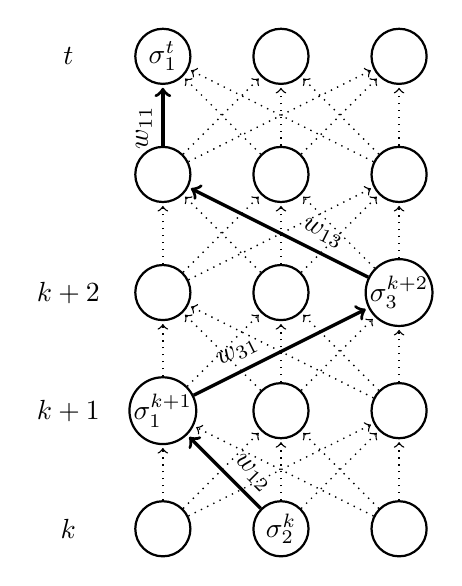
\begin{tikzpicture}[rnn_style]

  
  \node[neuron]    (x1)[]   {$\sigma_1^t$};
  \node[neuron]    (x2)[right of=x1]   {};
  \node[neuron]    (x3)[right of=x2]   {};
  \node[label]     (xl)[left of=x1] {$t$};
  
  \node[neuron]    (h1)[below of =x1]   {$\hdots$};
  \node[neuron]    (h2)[right of=h1]   {};
  \node[neuron]    (h3)[right of=h2]   {};
  \node[label]     (hl)[left of=h1] {$\hdots$};
  
  \node[neuron]    (y1)[below of=h1]   {};
  \node[neuron]    (y2)[right of=y1]   {};
  \node[neuron]    (y3)[right of=y2]   {$\sigma_3^{k+2}$};
  \node[label]     (yl)[left of=y1] {$k+2$};

  
  \node[neuron]    (z1)[below of=y1]   {$\sigma_1^{k+1}$};
  \node[neuron]    (z2)[right of=z1]   {};
  \node[neuron]    (z3)[right of=z2]   {};
  \node[label]     (zl)[left of=z1] {$k+1$};
  
  \node[neuron]    (w1)[below of=z1]   {};
  \node[neuron]    (w2)[right of=w1]   {$\sigma_2^k$};
  \node[neuron]    (w3)[right of=w2]   {};
  \node[label]     (wl)[left of=w1] {$k$};

  
%   \node[label]      (lu)[left of=u] {$u$};
%   \node[label]      (ll)[left of=z1] {$l$};


  \path[->] (h1) edge [thick_edge] node[weight]{$w_{11}$}  (x1)
	    (h1) edge [thin_edge]   (x2)
	    (h1) edge [thin_edge]   (x3)
	    (h2) edge [thin_edge]  (x1)
	    (h2) edge [thin_edge]   (x2)
	    (h2) edge [thin_edge]   (x3)
	    (h3) edge [thin_edge]  (x1)
	    (h3) edge [thin_edge]   (x2)
	    (h3) edge [thin_edge]   (x3);

  \path[->] (y1) edge [thin_edge]   (h1)
	    (y1) edge [thin_edge]   (h2)
	    (y1) edge [thin_edge]   (h3)
	    (y2) edge [thin_edge]   (h1)
	    (y2) edge [thin_edge]   (h2)
	    (y2) edge [thin_edge]   (h3)
	    (y3) edge [thick_edge] node[weight]{$w_{13}$}   (h1)
	    (y3) edge [thin_edge]   (h2)
	    (y3) edge [thin_edge]   (h3);
  
  
  \path[->] (z1) edge [thin_edge]   (y1)
	    (z1) edge [thin_edge]  (y2)
	    (z1) edge [thick_edge] node[weight]{$w_{31}$}   (y3)
	    (z2) edge [thin_edge]  (y1)
	    (z2) edge [thin_edge]  (y2)
	    (z2) edge [thin_edge]  (y3)
	    (z3) edge [thin_edge]   (y1)
	    (z3) edge [thin_edge]   (y2)
	    (z3) edge [thin_edge]   (y3);
	    
  \path[->] (w1) edge [thin_edge]   (z1)
	    (w1) edge [thin_edge]  (z2)
	    (w1) edge [thin_edge]   (z3)
	    (w2) edge [thick_edge] node[weight]{$w_{12}$}   (z1)
	    (w2) edge [thin_edge]   (z2)
	    (w2) edge [thin_edge]   (z3)
	    (w3) edge [thin_edge]   (z1)
	    (w3) edge [thin_edge]   (z2)
	    (w3) edge [thin_edge]   (z3);

	    


\end{tikzpicture}
\caption{The cost for a path from neuron $2$ at time $k$ to neuron $1$ at time $t$ is $w_{12}w_{31}w_{13}\hdots w_{11}\cdot \sigma_2^k \sigma_1^{k+1}\sigma_3^{k+2} \hdots \sigma_1^{t-1} $ }
\label{gradient_path_cost}
\end{figure}


We can further characterize each path cost noticing that we can separate two components, one that depends only on the weights $w_{qj} \hdots w_{jh}$ and the other that depends both on the weights and the inputs
$\sigma'(a_j^k)\sigma'(a_q^{k}) \hdots \sigma'(a_i^{t-1})$.


\paragraph{The ReLU case}
ReLU case is a bit special, because of it's derivative.
ReLU's derivative is a step function, it can assume only two values: $1$ when the neuron is active, $0$ otherwise.
Returning to the path graph we introduced earlier we can say that a path is \textit{enabled} if each neuron in that path is active. In fact if we
encounter a path which cross a non active neuron it's path cost will be 0; on the contrary for an \textit{enabled} path the cost will be simply the product
of weight of the arcs we went through, as we can see in figure \ref{gradient_path_cost_relu}


\tikzstyle{rnn_style}=[->,shorten >=1pt,auto,node distance=1.5cm,
  thick,
  neuron/.style={circle,fill=white!50,draw,minimum size=0.7cm,inner sep=0pt,font=\sffamily\normalsize},
  missing/.style={circle,fill=white!50,draw=none,minimum size=0.7cm,font=\sffamily\Huge\bfseries},
  label/.style={node distance=1.2cm,rectangle,fill=white!50,draw=none,minimum size=0.7cm,font=\sffamily\normalsize},
  thick_edge/.style={line width=1.2pt},
  thin_edge/.style={dotted, line width=0.5pt},
  weight/.style = {above,sloped,pos=0.3},
  blacked/.style={fill=black},
  ]
\begin{figure}
 \centering
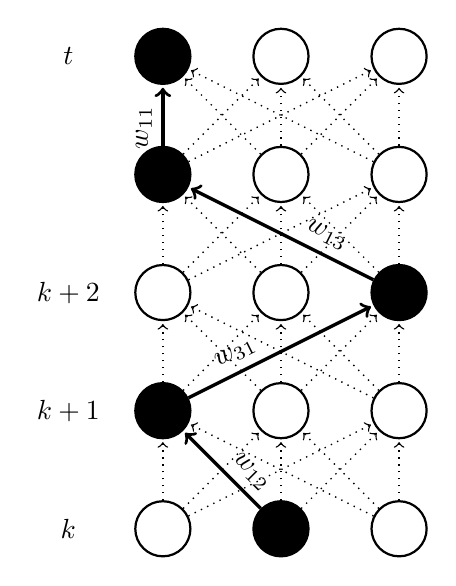
\begin{tikzpicture}[rnn_style]

  
  \node[neuron,blacked]    (x1)[]   {};
  \node[neuron]    (x2)[right of=x1]   {};
  \node[neuron]    (x3)[right of=x2]   {};
  \node[label]     (xl)[left of=x1] {$t$};
  
  \node[neuron,blacked]    (h1)[below of =x1]   {};
  \node[neuron]    (h2)[right of=h1]   {};
  \node[neuron]    (h3)[right of=h2]   {};
  \node[label]     (hl)[left of=h1] {$\hdots$};
  
  \node[neuron]    (y1)[below of=h1]   {};
  \node[neuron]    (y2)[right of=y1]   {};
  \node[neuron,blacked]    (y3)[right of=y2]   {};
  \node[label]     (yl)[left of=y1] {$k+2$};

  
  \node[neuron,blacked]    (z1)[below of=y1]   {};
  \node[neuron]    (z2)[right of=z1]   {};
  \node[neuron]    (z3)[right of=z2]   {};
  \node[label]     (zl)[left of=z1] {$k+1$};
  
  \node[neuron]    (w1)[below of=z1]   {};
  \node[neuron,blacked]    (w2)[right of=w1]   {};
  \node[neuron]    (w3)[right of=w2]   {};
  \node[label]     (wl)[left of=w1] {$k$};

  
%   \node[label]      (lu)[left of=u] {$u$};
%   \node[label]      (ll)[left of=z1] {$l$};


  \path[->] (h1) edge [thick_edge] node[weight]{$w_{11}$}  (x1)
	    (h1) edge [thin_edge]   (x2)
	    (h1) edge [thin_edge]   (x3)
	    (h2) edge [thin_edge]  (x1)
	    (h2) edge [thin_edge]   (x2)
	    (h2) edge [thin_edge]   (x3)
	    (h3) edge [thin_edge]  (x1)
	    (h3) edge [thin_edge]   (x2)
	    (h3) edge [thin_edge]   (x3);

  \path[->] (y1) edge [thin_edge]   (h1)
	    (y1) edge [thin_edge]   (h2)
	    (y1) edge [thin_edge]   (h3)
	    (y2) edge [thin_edge]   (h1)
	    (y2) edge [thin_edge]   (h2)
	    (y2) edge [thin_edge]   (h3)
	    (y3) edge [thick_edge] node[weight]{$w_{13}$}   (h1)
	    (y3) edge [thin_edge]   (h2)
	    (y3) edge [thin_edge]   (h3);
  
  
  \path[->] (z1) edge [thin_edge]   (y1)
	    (z1) edge [thin_edge]  (y2)
	    (z1) edge [thick_edge] node[weight]{$w_{31}$}   (y3)
	    (z2) edge [thin_edge]  (y1)
	    (z2) edge [thin_edge]  (y2)
	    (z2) edge [thin_edge]  (y3)
	    (z3) edge [thin_edge]   (y1)
	    (z3) edge [thin_edge]   (y2)
	    (z3) edge [thin_edge]   (y3);
	    
  \path[->] (w1) edge [thin_edge]   (z1)
	    (w1) edge [thin_edge]  (z2)
	    (w1) edge [thin_edge]   (z3)
	    (w2) edge [thick_edge] node[weight]{$w_{12}$}   (z1)
	    (w2) edge [thin_edge]   (z2)
	    (w2) edge [thin_edge]   (z3)
	    (w3) edge [thin_edge]   (z1)
	    (w3) edge [thin_edge]   (z2)
	    (w3) edge [thin_edge]   (z3);

	    


\end{tikzpicture}
\caption{The cost for an enabled path from neuron $2$ at time $k$ to neuron $1$ at time $t$ is $w_{12}w_{31}w_{13}\hdots w_{11}$ }
\label{gradient_path_cost_relu}
\end{figure}

So $\vert (\frac{\partial \vec{a}^t}{\partial \vec{a}^k})_{ij}\vert$ ranges from 0, when no path is enabled to, $\vert ((\mat{W}^{rec})^{t-k-1})_{ij} \vert$ when all
paths are enabled and all path cost have the same sign, which is consistent with what we found in Hochreiter analysis.
We can argue then that ReLU has an advantage over sigmoidal activation functions, for instance, because gradient depends only on the $\mat{W}^{rec}$ matrix:
ReLU function \textit{only} enables or disables the paths but doesn't change their costs as sigmoids do


\paragraph{Poor solutions}
Let's pretend we have found, with some learning technique, an assignment for all the weights which causes the gradient to have zero norm. We could be happy with
it and claim to have 'solved' the problem. However, by chance, we discover that $\frac{\partial \vec{a}^T}{\partial \vec{a}^k}$ has zero norm for all
time steps $k<\tau$. So, the output of the network doesn't depend on the inputs of the sequence for those time steps.
In other words we have found a possibly optimal solution for the truncated sequence ${x}_{[\tau:T]}$. The solution we have found is an optimal candidate to
be a bad local minimum.

As a final observation on this topic it's worth noticing how a bad initialization of $\mat{W^{rec}}$ can lead to poor solutions or extremely large convergence time
just because such initialization imply $\frac{\partial \vec{a}^t}{\partial \vec{a}^k}$ approaching zero norm for $t\gg k$. Moreover, even if we somehow provide
an initialization matrix which is unaffected by this curse, it's certainly possible that we reach such a bad matrix during learning phase.
Several techniques have been proposed to overcome this problem, they will be the topic of later chapters.





